\documentclass{class}

\addbibresource{bib.bib}

\title{Dictyostelium Chemotaxis}
\author{Florian Lang 11711870}
\date{25.08.2022}

\begin{document}

\maketitle

\begin{abstract}
In this project we through the model proposed in \cite{paper}.
It models the aggregation of \emph{Dictyostelium discoideum} cells into larger structures which happens through chemical communication.
We will not look at external sources of the chemical, only those emitted by the cells.
As the case of an initial uniform distribution and differing parameters has already been look at (and can be looked at at \href{https://www.complexity-explorables.org/explorables/come-together/}{Complexity Explorables}), we will look at different initial particle distributions and different configurations of so called pacemakers, i.e. special cells that emit the chemical at regular frequency regardless of other parameters.
\end{abstract}

\section{Idea}

Essentially the cells want to aggregate in to larger structures and they do so via chemical interaction.
They try to detect the chemical in their surrounding.
If they detect some, they move in the direction of the highest concentration and switch into an active state.
In their active state they emit the chemical by themselves so other particles can find them as well.
After some time in the active state the cell has to recover and switches into an recovering state in which the cell does nothing.
When the cell recovers it goes back to try detecting the chemical.

To get this whole process starting there are special pacemaker cells which simply skip the detecting of the chemical.
So pacemaker cells simply emit the chemical at a fixed frequency and hence are some sort of a beacon for the other particles.

\section{Model}

The \emph{concentration of the chemical} is modelled by a function
\begin{align*}
    C:\ 
    \R^3&\to\R\\
    (x,\,y,\,t)&\mapsto C(x,\,y,\,t).
\end{align*}
The \emph{cells} (in the following \emph{particles}) are modelled by
\begin{align*}
    p_i=(x_i,\,y_i,\,s_i)\in\R^3,\quad i\in\{1,\,2,\,\ldots,\,N\}.
\end{align*}
where $(x_i,\,y_i)$ is the location while $s_i$ is the current state of the particle.
Essentially the particles have 3 different states.
\begin{itemize}
    \item \emph{Active}, while which the particle emits the chemical at a rate $\gamma$.
          The particle is in this state for a time $t_a$ and then it switches to the \emph{recovering} state.
    \item \emph{Recovering}, while which the particle does nothing for some time $t_r$ and then it switches to the
          \emph{inactive} state.
    \item \emph{Inactive}, while which the particle tries to detect the chemical in its surrounding.
          If there is a concentration larger than some threshold $\tau$, the particle moves a fixed distance $d$ in the direction of the largest concentration
          \begin{align*}
              (x_i,\,y_i)\rightarrow(x_i,\,y_i)+\frac{\nabla C}{\norm{\nabla C}}d,
          \end{align*}
          if the gradient is larger than some threshold $m$, and it switches into the \emph{active} state.
\end{itemize}
Besides the movement in the direction of the highest concentration the particles also move randomly with a magnitude $r$.
For a more convenient way to look at the particle states see the flow chart in \autoref{fig:states}.
\begin{figure}
    \centering
    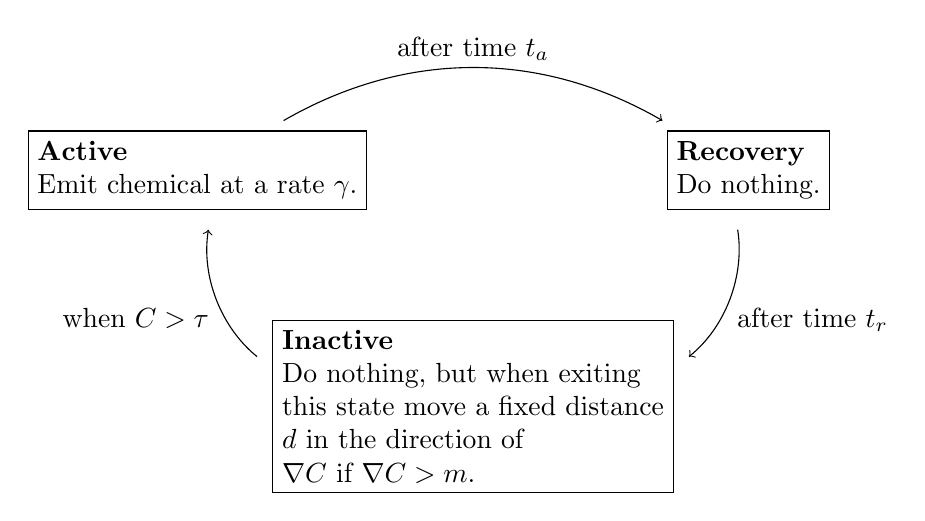
\begin{tikzpicture}
        \node[
            draw,
            minimum width=2cm,
            minimum height=1cm,
            align=left
        ] (A) at (0,0)
        {
            \textbf{Active}\\
            Emit chemical at a rate $\gamma$.
        };
        \node[
            draw,
            minimum width=2cm,
            minimum height=1cm,
            align=left
        ] (R) at (7,0)
        {
            \textbf{Recovery}\\
            Do nothing.
        };
        \node[
            draw,
            minimum width=2cm,
            minimum height=1cm,
            align=left
        ] (I) at (3.5,-3)
        {
            \textbf{Inactive}\\
            Do nothing, but when exiting\\
            this state move a fixed distance\\
            $d$ in the direction of\\
            $\nabla C$ if $\norm{\nabla C}>m$.
        };
        \draw[->,shorten >=0.25cm,shorten <=0.25cm] (A) to[edge label=after time $t_a$, bend left] (R);
        \draw[->,shorten >=0.25cm,shorten <=0.25cm] (R) to[edge label=after time $t_r$, bend left] (I);
        \draw[->,shorten >=0.25cm,shorten <=0.25cm] (I) to[edge label=when $C>\tau$, bend left] (A);
    \end{tikzpicture}
    \caption{Particle States}
    \label{fig:states}
\end{figure}

Apart from the emission of the particles the concentration is naturally object to diffusion at a rate $\alpha$ and decay at a rate $\beta$.
So all in all we get for the concentration
\begin{align}\label{eq:C}
    \pdv{C}{t}=\alpha\left(\pdv[2]{C}{x}+\pdv[2]{C}{y}\right)-\beta C+\sum_{a\in A}\gamma_a\delta_a.
\end{align}
Where the first term describes the diffusion, the second term the decay and the last term describes the newly emitted chemical of the currently active particles $A$.
Note that $\delta_a$ is a delta distribution centered at the position of the particle $a$ and $\gamma_a$ is the emission rate of the particle $a$.

To get the whole process starting we introduce \emph{pacemaker} particles which act similar to normal particles except that they have a different emission rate $\gamma_p$ and they skip the inactive state and go directly from recovering to active.

Note that for every cycle of a particle the non-random movement is similar to a gradient flow where $C$ acts as the potential.

\subsection{Some Comments On Modelling Choices}

Now let us discuss some of the choices made.

First the 3 states come from the assumption that a cell doesn't have an infinite supply of the chemical, so after it emitted a bunch, it has to recover, i.e. produce some of the chemical again.

Secondly we assume that both the detection of the concentration as well as the detection of the concentration gradient must have some threshold as the cells cannot detect too little changes in either.

Further we assumed that all the cell specific constants (like the times in states or the thresholds) vary very little from cell to cell so we can set the same parameters for all the cells.

We naturally assumed that the chemical diffuses.
We also assumed that by some chemical process (for example oxidisation) the chemical decays after some time.
Both the decay an diffusion we assumed to happen homogeneous throughout space and time.

The choices for the initial particle distributions we will look at later mostly lack motivation, however there might be reasons for such initial distributions to occur for example differing fluid viscosity or other obstructions in the domain.

Also note that this model does not consider collisions of particles and it will possibly fail to model reality if the particle density gets to high.

\section{Kinetic Equation}

Sadly we were not able to formulate the the particle movement and the state dynamics in a more formal way, let alone derive the kinetic equation, as the problem was to complex to handle for us (if it is even possible in a time continuous way).

\section{Dimensional Analysis}

Note that $\alpha$ has dimension $length^2\cdot time^{-1}$, $\beta$ has dimension $time^{-1}$ and $\gamma_a$ has dimension $concentration\cdot time^{-1}$.
If we were to introduce the unit-less variables $v=x\sqrt{\frac{\beta}{\alpha}},\,w=y\sqrt{\frac{\beta}{\alpha}},\,s=\beta t$ and use $\tau$ as reference concentration we could define
\begin{align*}
    \C(v,\,w,\,s)=\frac{1}{\tau}C\left(\sqrt{\frac{\alpha}{\beta}}v,\,\sqrt{\frac{\alpha}{\beta}}w,\,\frac{s}{\beta}\right).
\end{align*}
This then gives
\begin{align*}
    \C_{vv}(v,\,w,\,s)
    &=\frac{\alpha}{\tau\beta}C_{xx}\left(\sqrt{\frac{\alpha}{\beta}}v,\,\sqrt{\frac{\alpha}{\beta}}w,\,\frac{s}{\beta}\right)\\
    \C_{ww}(v,\,w,\,s)
    &=\frac{\alpha}{\tau\beta}C_{yy}\left(\sqrt{\frac{\alpha}{\beta}}v,\,\sqrt{\frac{\alpha}{\beta}}w,\,\frac{s}{\beta}\right)\\
    \C_{s}(v,\,w,\,s)
    &=\frac{1}{\tau\beta}C_{t}\left(\sqrt{\frac{\alpha}{\beta}}v,\,\sqrt{\frac{\alpha}{\beta}}w,\,\frac{s}{\beta}\right).
\end{align*}
Using \autoref{eq:C} we would get 
\begin{align*}
    \C_s(v,\,w,\,s)
    =&\,\frac{1}{\tau\beta}C_{t}\left(\sqrt{\frac{\alpha}{\beta}}v,\,\sqrt{\frac{\alpha}{\beta}}w,\,\frac{s}{\beta}\right)\\
    =&\,\frac{1}{\tau\beta}\Bigg(\alpha\left(C_{xx}\left(\sqrt{\frac{\alpha}{\beta}}v,\,\sqrt{\frac{\alpha}{\beta}}w,\,\frac{s}{\beta}\right)+C_{yy}\left(\sqrt{\frac{\alpha}{\beta}}v,\,\sqrt{\frac{\alpha}{\beta}}w,\,\frac{s}{\beta}\right)\right)\\
    &\,-\beta C\left(\sqrt{\frac{\alpha}{\beta}}v,\,\sqrt{\frac{\alpha}{\beta}}w,\,\frac{s}{\beta}\right)+\sum_{a\in A}\gamma_a\delta_a\Bigg)\\
    =&\,\C_{vv}(v,\,w,\,s)+\C_{ww}(v,\,w,\,s)-\C(v,\,w,\,s)+\sum_{a\in A}\tilde{\gamma}_a\delta_a
\end{align*}
with $\tilde{\gamma}_a=\frac{\gamma_a}{\tau\beta}$.
This equation is now completely unit-less.
However we will stick to the equation with units for the following.

\section{Implementation}

To simulate the concentration $C$ we use a discrete square grid.
We choose the grid larger than the area in which particles are found, so we essentially model a theoretically unbounded domain but with a bounded space in which the particles are.
This means we do not need to think about boundary conditions.

The particle state is modelled trough a float.
If it is positive then the particle is currently active.
If it is negative then the particle is recovering.
Finally the state $0$ corresponds to an inactive particle.

We will now go through what is done in a single time step of the simulation.

Note that we will use a temporary emitted concentration variable $C_e$ to keep track of the total amount of newly emitted chemical, to avoid particle interactions in the same time step.

The particle dynamics is easily implemented as follows.
\begin{itemize}
    \item If the particle is at state $0$ and the concentration $C$ in its underlying grid cell above $\tau$ its state gets set to $t_a$.
    If $\norm{\nabla C}>m$ then also update the particle location with $(x_i,\,y_i)\rightarrow(x_i,\,y_i)+\frac{\nabla C}{\norm{\nabla C}}d$
    \item If the particle state is positive then decrement the particle state by $\Delta t$ (or set it to $-t_r$ if it would get negative).
    Also increment the emitted concentration $C_e$ by $\Delta t\gamma$ in the cell corresponding to the particles position.
    \item If the particle state is negative then increment the state by $\Delta t$ (or set it to $0$ if it would get positive).
\end{itemize}

For pacemaker particles we have similarly
\begin{itemize}
    \item If the particle state is positive then decrement the particle state by $\Delta t$ (or set it to $-t_r$ if it would get negative).
    Also increment the emitted concentration $C_e$ by $\Delta t\gamma_p$ in the cell corresponding to the particles position.
    \item If the particle state is negative then increment the state by $\Delta t$ (or set it to $t_a$ if it would get positive).
\end{itemize}

After we have done this $C_e$ corresponds to $\Delta t\sum_{a\in A}\gamma_a\delta_a$ in \autoref{eq:C} which we can now add to $C$.

Now its left to do the diffusion and decay part of \autoref{eq:C}, i.e.
\begin{align*}
    \pdv{C}{t}=\alpha\left(\pdv[2]{C}{x}+\pdv[2]{C}{y}\right)-\beta C.
\end{align*}
We use the implicit Euler method for doing this time step. The equation hence reads
\begin{align*}
    \frac{C^{n+1}_{i,j}-C^n_{i,j}}{\Delta t}
    =\alpha\left(\frac{C^{n+1}_{i-1,j}-2C^{n+1}_{i,j}+C^{n+1}_{i+1,j}}{\Delta x^2}+\frac{C^{n+1}_{i,j-1}-2C^{n+1}_{i,j}+C^{n+1}_{i,j+1}}{\Delta x^2}\right)-\beta C^{n+1}_{i,j}
\end{align*}
or rearranged
\begin{align*}
    C^n_{i,j}
    =\left(1+4\frac{\Delta t\alpha}{\Delta x^2}+\Delta t\beta\right)C^{n+1}_{i,j}-\frac{\Delta t\alpha}{\Delta x^2}C^{n+1}_{i-1,j}-\frac{\Delta t\alpha}{\Delta x^2}C^{n+1}_{i+1,j}-\frac{\Delta t\alpha}{\Delta x^2}C^{n+1}_{i,j-1}-\frac{\Delta t\alpha}{\Delta x^2}C^{n+1}_{i,j+1}.
\end{align*}
So writing $C^n$ as a vector in an appropriate way gives
\begin{align*}
    C^n=AC^{n+1}
\end{align*}
where $A$ is a sparse matrix and we only need to solve this linear equation for $C^{n+1}$.

Finally we only need to change the particle position by a small (determined by the \emph{random magnitude} $r$) random value.

\section{Simulations And Observations}

In \autoref{tab:par} are the parameters we used and did not change for the following simulations.
Only the initial distribution of particles changes throughout the different simulations.
\begin{table}
    \centering
    \begin{tabular}{l|l|r}
        Parameter  & Description & Value\\\hline\hline
        $N$        & Number of cells & 5000\\\hline
        $S$        & Width and height of the square & 10\\\hline
        $\Delta x$ & Spacing of the grid & 0.1\\\hline
        $\Delta t$ & Time step & 0.0006\\\hline
        $\alpha$   & Diffusion rate & 3\\\hline
        $\beta$    & Decay rate & 32\\\hline
        $t_a$      & Time in \emph{active} state & 0.004\\\hline
        $t_r$      & Time in \emph{recovery} state & 0.06\\\hline
        $\gamma$   & Emission rate & 6000\\\hline
        $\gamma_p$ & Emission rate for pacemakers & 15000\\\hline
        $\tau$     & Chemical detection threshold & 1.5\\\hline
        $r$        & Random movement magnitude & 0.03\\\hline
        $d$        & Moving distance & 0.03\\\hline
        $m$        & Movement threshold & 1\\\hline
    \end{tabular}
    \caption{Parameter Descriptions}
    \label{tab:par}
\end{table}

\begin{minipage}{0.55\textwidth}
\begin{align*}
\includegraphics[width=0.49\textwidth]{simulation/1/frame_0.png}\hfill
\includegraphics[width=0.49\textwidth]{simulation/1/frame_71.png}
\\[\smallskipamount]
\includegraphics[width=0.49\textwidth]{simulation/1/frame_143.png}\hfill
\includegraphics[width=0.49\textwidth]{simulation/1/frame_214.png}
\\[\smallskipamount]
\includegraphics[width=0.49\textwidth]{simulation/1/frame_285.png}\hfill
\includegraphics[width=0.49\textwidth]{simulation/1/frame_356.png}
\\[\smallskipamount]
\includegraphics[width=0.49\textwidth]{simulation/1/frame_428.png}\hfill
\includegraphics[width=0.49\textwidth]{simulation/1/frame_499.png}
\end{align*}
\end{minipage}
\begin{minipage}{0.45\textwidth}
\subsection{Annulus}
In our first simulation we used an uniform distribution on an annulus.
A pattern emerges after about $1$s.
It is apparent that the missing particles in the middle prevent any interaction through the hole which gives rise to branches above and below the hole, displaying a nice symmetry.
One can also observe that where the two \lq{}concentration fronts\rq{} collide on the right, a clear separation of the particles takes place.
\end{minipage}
\begin{minipage}{0.55\textwidth}
\begin{align*}
\includegraphics[width=0.49\textwidth]{simulation/2/frame_0.png}\hfill
\includegraphics[width=0.49\textwidth]{simulation/2/frame_71.png}
\\[\smallskipamount]
\includegraphics[width=0.49\textwidth]{simulation/2/frame_143.png}\hfill
\includegraphics[width=0.49\textwidth]{simulation/2/frame_214.png}
\\[\smallskipamount]
\includegraphics[width=0.49\textwidth]{simulation/2/frame_285.png}\hfill
\includegraphics[width=0.49\textwidth]{simulation/2/frame_356.png}
\\[\smallskipamount]
\includegraphics[width=0.49\textwidth]{simulation/2/frame_428.png}\hfill
\includegraphics[width=0.49\textwidth]{simulation/2/frame_499.png}
\end{align*}
\end{minipage}
\begin{minipage}{0.45\textwidth}
\subsection{High Density Center}
Here we use a disk with a higher density of particles in its center and an offset pacemaker.
Again a pattern is clearly visible at about $1$s.
The dense center does not seem to affect the spread of the chemical.
After about $2.5$s this high density area transforms into a a slightly thicker, but more or less indistinguishable, branch of the pattern.
\end{minipage}
\begin{minipage}{0.55\textwidth}
\begin{align*}
\includegraphics[width=0.49\textwidth]{simulation/6/frame_0.png}\hfill
\includegraphics[width=0.49\textwidth]{simulation/6/frame_71.png}
\\[\smallskipamount]
\includegraphics[width=0.49\textwidth]{simulation/6/frame_143.png}\hfill
\includegraphics[width=0.49\textwidth]{simulation/6/frame_214.png}
\\[\smallskipamount]
\includegraphics[width=0.49\textwidth]{simulation/6/frame_285.png}\hfill
\includegraphics[width=0.49\textwidth]{simulation/6/frame_356.png}
\\[\smallskipamount]
\includegraphics[width=0.49\textwidth]{simulation/6/frame_428.png}\hfill
\includegraphics[width=0.49\textwidth]{simulation/6/frame_499.png}
\end{align*}
\end{minipage}
\begin{minipage}{0.45\textwidth}
\subsection{Even Higher Density Center}
Here we use a disk with a even higher density of particles and the dense center still does not seem to affect the spread of the chemical.
However this time the high density area is still present at the end of the simulation as a thick branch.
\end{minipage}
\begin{minipage}{0.55\textwidth}
\begin{align*}
\includegraphics[width=0.49\textwidth]{simulation/3/frame_0.png}\hfill
\includegraphics[width=0.49\textwidth]{simulation/3/frame_71.png}
\\[\smallskipamount]
\includegraphics[width=0.49\textwidth]{simulation/3/frame_143.png}\hfill
\includegraphics[width=0.49\textwidth]{simulation/3/frame_214.png}
\\[\smallskipamount]
\includegraphics[width=0.49\textwidth]{simulation/3/frame_285.png}\hfill
\includegraphics[width=0.49\textwidth]{simulation/3/frame_356.png}
\\[\smallskipamount]
\includegraphics[width=0.49\textwidth]{simulation/3/frame_428.png}\hfill
\includegraphics[width=0.49\textwidth]{simulation/3/frame_499.png}
\end{align*}
\end{minipage}
\begin{minipage}{0.45\textwidth}
\subsection{Low Density Center}
Contrary to the previous we used a disk with a lower density in the center in this simulation.
Again a pattern is clearly visible at about $1$s.
One can observe a very similar pattern to the Annulus simulation, a few branches going above the center and a few going below, but none going through.
The chemical diffusion clearly seems to prefer higher particle densities for its distribution.
Also similar to the annulus simulation we get a separation at the right.
\end{minipage}
\begin{minipage}{0.55\textwidth}
\begin{align*}
\includegraphics[width=0.49\textwidth]{simulation/4/frame_0.png}\hfill
\includegraphics[width=0.49\textwidth]{simulation/4/frame_71.png}
\\[\smallskipamount]
\includegraphics[width=0.49\textwidth]{simulation/4/frame_143.png}\hfill
\includegraphics[width=0.49\textwidth]{simulation/4/frame_214.png}
\\[\smallskipamount]
\includegraphics[width=0.49\textwidth]{simulation/4/frame_285.png}\hfill
\includegraphics[width=0.49\textwidth]{simulation/4/frame_356.png}
\\[\smallskipamount]
\includegraphics[width=0.49\textwidth]{simulation/4/frame_428.png}\hfill
\includegraphics[width=0.49\textwidth]{simulation/4/frame_499.png}
\end{align*}
\end{minipage}
\begin{minipage}{0.45\textwidth}
\subsection{Even Lower Density Center}
To take the Low Density Center simulation to the extreme we further lowered the center density here.
Again we get a similar result to the Annulus simulation.
Compared to the Low Density Simulation a even more pronounced empty circle in the center emerges.
Because of the low density there are even a few particles (the grey ones) that never left their inactive state as they where never in reach of the chemical.
Note that the separation on the right is way more visible compared to the Low Density Center simulation.
\end{minipage}
\begin{minipage}{0.55\textwidth}
\begin{align*}
\includegraphics[width=0.49\textwidth]{simulation/5/frame_0.png}\hfill
\includegraphics[width=0.49\textwidth]{simulation/5/frame_143.png}
\\[\smallskipamount]
\includegraphics[width=0.49\textwidth]{simulation/5/frame_285.png}\hfill
\includegraphics[width=0.49\textwidth]{simulation/5/frame_428.png}
\\[\smallskipamount]
\includegraphics[width=0.49\textwidth]{simulation/5/frame_571.png}\hfill
\includegraphics[width=0.49\textwidth]{simulation/5/frame_714.png}
\\[\smallskipamount]
\includegraphics[width=0.49\textwidth]{simulation/5/frame_856.png}\hfill
\includegraphics[width=0.49\textwidth]{simulation/5/frame_999.png}
\end{align*}
\end{minipage}
\begin{minipage}{0.45\textwidth}
\subsection{Sine Wave}
Here we used a distribution that resembles a sine curve to see how the chemical gets around sharper edges.
It appears that the particle chain breaks if there is a sharp turn involved.
We end up with \lq{}self-powered\rq{} blobs corresponding to the extrema of the sine wave.
\end{minipage}
\begin{minipage}{0.55\textwidth}
\begin{align*}
\includegraphics[width=0.49\textwidth]{simulation/7/frame_0.png}\hfill
\includegraphics[width=0.49\textwidth]{simulation/7/frame_119.png}
\\[\smallskipamount]
\includegraphics[width=0.49\textwidth]{simulation/7/frame_238.png}\hfill
\includegraphics[width=0.49\textwidth]{simulation/7/frame_357.png}
\\[\smallskipamount]
\includegraphics[width=0.49\textwidth]{simulation/7/frame_476.png}\hfill
\includegraphics[width=0.49\textwidth]{simulation/7/frame_595.png}
\\[\smallskipamount]
\includegraphics[width=0.49\textwidth]{simulation/7/frame_713.png}\hfill
\includegraphics[width=0.49\textwidth]{simulation/7/frame_832.png}
\end{align*}
\end{minipage}
\begin{minipage}{0.45\textwidth}
\subsection{In Sync Pacemakers}
Here we tried a uniform distribution on a square but having two pacemakers which are running in sync.
One can observe that similar to the case of the Annulus we have a clear separation where the two concentration fronts collide.
This leads to a clear and straight separation of the two structures which are of a similar size.
\end{minipage}
\begin{minipage}{0.55\textwidth}
\begin{align*}
\includegraphics[width=0.49\textwidth]{simulation/8/frame_0.png}\hfill
\includegraphics[width=0.49\textwidth]{simulation/8/frame_119.png}
\\[\smallskipamount]
\includegraphics[width=0.49\textwidth]{simulation/8/frame_238.png}\hfill
\includegraphics[width=0.49\textwidth]{simulation/8/frame_357.png}
\\[\smallskipamount]
\includegraphics[width=0.49\textwidth]{simulation/8/frame_476.png}\hfill
\includegraphics[width=0.49\textwidth]{simulation/8/frame_595.png}
\\[\smallskipamount]
\includegraphics[width=0.49\textwidth]{simulation/8/frame_713.png}\hfill
\includegraphics[width=0.49\textwidth]{simulation/8/frame_832.png}
\end{align*}
\end{minipage}
\begin{minipage}{0.45\textwidth}
\subsection{Out Of Sync Pacemakers}
Similar to the In Sync Pacemakers simulations we have a uniform distribution with two pacemakers.
This time we delayed the right pacemaker.
What one can observe is again very similar to the previous simulations.
At the place of the front collision a separation starts to form, however this time it is not a straight line but a hyperbola.
Also note that because the left pacemaker started early it had more time to \lq{}grab\rq{} particles and hence its structure is significantly bigger than the one to the right.
\end{minipage}

\subsection{Summary}

It is quite apparent that the chemical winds its way through batches of higher particle density, not even getting through areas in which the particle density is too low.

Whenever fronts of the chemical collide a separation in the structure(s) forms, in the case of multiple pacemakers this favours pacemakers which \lq{}fired\rq{} first.

If there are sharp turns in the particle distribution the structure might break more easily and form self-powered blobs.
These self-powered blobs contain particles in offset states, hence they are able to keep up a certain concentration in their surrounding and they activate each other.

\section{Possible Modifications}

\subsection{Random State Durations}

Instead of having fixed times in the active and recovery states one could look at exponentially distributed times with parameters $t_a^{-1}$ and $t_r^{-1}$ turning it in a continuous-time Markov Chain.

\subsection{Competing Particle Types}

Consider two different particle types which communicate through different chemicals which compete against each other.
So we would have something like
\begin{align*}
    \pdv{C_1}{t}
    &=\alpha\left(\pdv[2]{C_1}{x}+\pdv[2]{C_1}{y}\right)-\beta C_1+\sum_{a\in A_1}\gamma_a\delta_a-\lambda C_1C_2\\
    \pdv{C_2}{t}
    &=\alpha\left(\pdv[2]{C_2}{x}+\pdv[2]{C_2}{y}\right)-\beta C_2+\sum_{a\in A_2}\gamma_a\delta_a-\lambda C_1C_2.
\end{align*}
where we introduce the annihilation term $-\lambda C_1C_2$ which might model some chemical process between the two chemicals.

\subsection{More Dimensions}

In many scenarios it makes sense to look at this simulation in 2D, think about thin films of liquid in which the particles float in.
But it might also be of interest to observe this behaviour not in $\R^2$ but in $\R^3$ which requires minimal changes and gives
\begin{align*}
    \pdv{C}{t}
    &=\alpha\left(\pdv[2]{C}{x}+\pdv[2]{C}{y}+\pdv[2]{C}{z}\right)-\beta C+\sum_{a\in A}\gamma_a\delta_a.
\end{align*}

\subsection{External Influence}

Further one might also consider external chemical sources or drains which could be modelled by a function
\begin{align*}
    E:\ 
    \R^3&\to\R\\
    (x,\,y,\,t)&\mapsto E(x,\,y,\,t),
\end{align*}
and
\begin{align*}
    \pdv{C}{t}
    &=\alpha\left(\pdv[2]{C}{x}+\pdv[2]{C}{y}\right)-\beta C+\sum_{a\in A}\gamma_a\delta_a+E(x,\,y,\,t).
\end{align*}

\appendix

\printbibliography

\section{Appendix}

For reasons we have the python code displayed below, feel free to fiddle arround with it.
It is not perfectly commentated but it is something.

\subsection{chemotaxis.py}

\begin{minted}[fontsize=\scriptsize]{python}
import imageio
import matplotlib
import matplotlib.pyplot
import matplotlib.animation
import numpy as np
import os
import scipy.sparse
import scipy.sparse.linalg
from time import time

from tex import *
from parameters import *

# do a simulation for given parameters
def simulation(animation_name, N, size, dx, dt, alpha, beta, t_a, t_r, gamma, gamma_pacemaker, tau, movement_random,
               movement_distance, movement_threshold, T, pacemakers, distribution, time_steps_per_frame, dpi):
  global C, particle_locations, particle_states, pacemaker_locations, pacemaker_states
  gridsize = int(size / dx)

  # setup for the solver of the implicit euler step
  up =     - np.ones(gridsize * gridsize - gridsize)   * dt * alpha / (dx ** 2)      # cell up
  left =   - np.ones(gridsize * gridsize - 1)          * dt * alpha / (dx ** 2)      # cell to the left
  center =   np.ones(gridsize * gridsize) * (4 * alpha / (dx ** 2) + beta) * dt + 1  # main
  right =  - np.ones(gridsize * gridsize - 1)          * dt * alpha / (dx ** 2)      # cell to the right
  down =   - np.ones(gridsize * gridsize - gridsize)   * dt * alpha / (dx ** 2)      # cell down
  left[::gridsize] = 0
  right[-1::-gridsize] = 0
  A = scipy.sparse.diags([up, left, center, right, down], [-gridsize, -1, 0, 1, gridsize], format='csc')
  solver = scipy.sparse.linalg.factorized(A)

  # setup concentration and particles
  C = np.zeros((gridsize, gridsize))
  particle_locations = distribution
  particle_states = np.zeros(N)

  # setup pacemakers
  pacemaker_locations = np.array([pacemaker[:2] for pacemaker in pacemakers])
  pacemaker_states = np.array([pacemaker[2] for pacemaker in pacemakers])

  # do one time step
  def do_time_step():
    global C, particle_locations, particle_states, pacemaker_locations, pacemaker_states

    # get cell indices the particles and the pacemaker particles are in
    particle_indices = np.clip(np.round(particle_locations / dx).astype(int), 0, gridsize - 1)
    pacemaker_indices = np.clip(np.round(pacemaker_locations / dx).astype(int), 0, gridsize - 1)

    C_emitted = np.zeros((gridsize, gridsize))

    # calculate the gradient and the gradient norm of the concentration
    gradient_direction = np.zeros((gridsize, gridsize, 2))
    gradient_direction[1:-1, 1:-1, 0] = (C[2:, 1:-1] - C[:-2, 1:-1]) / (2 * dx)
    gradient_direction[1:-1, 1:-1, 1] = (C[1:-1, 2:] - C[1:-1, :-2]) / (2 * dx)
    gradient_norm = np.sqrt(gradient_direction[:, :, 0] ** 2 + gradient_direction[:, :, 1] ** 2)
    gradient_norm[gradient_norm == 0] = 1
    gradient_direction[:,:,0] = gradient_direction[:,:,0] / gradient_norm
    gradient_direction[:,:,1] = gradient_direction[:,:,1] / gradient_norm
    particle_gradient_norm = gradient_norm[(particle_indices.T[0], particle_indices.T[1])]
    particle_gradient_direction = gradient_direction[(particle_indices.T[0], particle_indices.T[1])]

    # get the particles of given states
    active_particles = particle_states > 0
    recovering_particles = particle_states < 0
    inactive_particles = particle_states == 0
    activating_particles = inactive_particles * (C[particle_indices.T[0], particle_indices.T[1]] > tau)
    moving_particles = activating_particles * (particle_gradient_norm > movement_threshold)

    # activate and move particles which are above the threshold
    particle_states[activating_particles] = t_a
    particle_locations[moving_particles] += movement_distance * particle_gradient_direction[moving_particles]

    # update and emit from active particles
    particle_states[active_particles] -= dt
    particle_states[active_particles * (particle_states <= 0)] = -t_r
    C_emitted[particle_indices[active_particles].T[0], particle_indices[active_particles].T[1]] += gamma * dt
    
    # update recovering particles
    particle_states[recovering_particles] += dt
    particle_states[recovering_particles * (particle_states > 0)] = 0

    # get the pacemaker particles of given states
    active_pacemakers = pacemaker_states >= 0
    recovering_pacemakers = pacemaker_states < 0

    # update and emit from active pacemaker particles
    pacemaker_states[active_pacemakers] -= dt
    pacemaker_states[active_pacemakers * (pacemaker_states < 0)] = -t_r
    C_emitted[pacemaker_indices[active_pacemakers].T[0], pacemaker_indices[active_pacemakers].T[1]] += gamma_pacemaker * dt

    # update recovering pacemaker particles
    pacemaker_states[recovering_pacemakers] += dt
    pacemaker_states[recovering_pacemakers * (pacemaker_states >= 0)] = t_a

    # move particles randomly
    particle_locations += (np.random.rand(N, 2) * 2 - 1) * movement_random * np.sqrt(dt)

    # update C with emitted C alpha and diffuse
    C += C_emitted
    C = solver(C.flatten()).reshape(gridsize, gridsize)
    return active_particles, recovering_particles, inactive_particles


  # animation setup
  colors = matplotlib.colors.LinearSegmentedColormap.from_list('C', ['white', 'blue'])
  fig, ax = matplotlib.pyplot.subplots()
  c_plot = matplotlib.pyplot.imshow(C.T, vmin=0, vmax=16, cmap=colors, interpolation='bilinear')
  active_particles_plot, = matplotlib.pyplot.plot([], [], 'bo', ms=1)
  inactive_particles_plot, = matplotlib.pyplot.plot([], [], 'ko', ms=1, alpha=0.2)
  recovering_particles_plot, = matplotlib.pyplot.plot([], [], 'ko', ms=1)
  pacemaker_plot, = matplotlib.pyplot.plot([], [], 'yo', ms=2)

  def init():
    ax.set_xlim([1, gridsize])
    ax.set_ylim([gridsize, 1])

  def update(i):
    # do the time step
    for _ in range(time_steps_per_frame - 1):
      do_time_step()
    active, recovering, inactive = do_time_step()

    # plot particles and the concentration
    ax.axis('off')
    ax.set_title('{:.3f} s'.format(i * dt * time_steps_per_frame))
    c_plot.set_data(C.T)
    active_particles_plot.set_data(particle_locations[active,0] / dx, particle_locations[active,1] / dx)
    inactive_particles_plot.set_data(particle_locations[inactive,0] / dx, particle_locations[inactive,1] / dx)
    recovering_particles_plot.set_data(particle_locations[recovering,0] / dx, particle_locations[recovering,1] / dx)
    pacemaker_plot.set_data(pacemaker_locations[:,0] / dx, pacemaker_locations[:,1] / dx)

  # do and animate the simulation
  animation = matplotlib.animation.FuncAnimation(fig, update, init_func=init, frames=int(T / (dt * time_steps_per_frame)),
                                                 repeat=True, interval=1, blit=False)
  animation.save(animation_name, fps=30, writer='imagemagick', dpi=dpi)


# run simulations for the parameters given in the parameters file
def main():
  global parameters
  start_point = 1
  for i, parameters in enumerate(parameters[start_point - 1:]):
    # create folder for this simulation if it doesn't exist yet
    folder = 'simulation/{}'.format(i + start_point)
    if not os.path.exists(folder):
      os.makedirs(folder)
    
    # clear folder
    for file in os.listdir(folder):
      os.remove(os.path.join(folder, file))

    # run simulation
    start = time()
    print('Simulating {}'.format(i + start_point))
    simulation(os.path.join(folder, 'animation.gif'), **parameters)
    print('Done in {} s'.format(time() - start))

    # extract a few frames of the animation and save it as a png
    frames = np.round(np.linspace(0, parameters['T'] / (parameters['dt'] * parameters['time_steps_per_frame']) - 1, 8)).astype(int)
    with imageio.get_reader(os.path.join(folder, 'animation.gif')) as reader:
      for frame in frames:
        image = reader.get_data(frame)
        # crop the image
        image = image[25:415, 145:515, :]
        imageio.imwrite(os.path.join(folder, 'frame_{}.png'.format(frame)), image)
    print('Saved images')

    # save tex output to folder
    with open(os.path.join(folder, 'tex.tex'), 'w') as f:
      f.write(tex([os.path.join(folder, 'frame_{}.png'.format(frame)) for frame in frames]))

main()
\end{minted}

\subsection{tex.py}

\begin{minted}[fontsize=\scriptsize]{python}
image_template = '''\\includegraphics[width=0.49\\textwidth]{{{}}}\\hfill
\\includegraphics[width=0.49\\textwidth]{{{}}}
\\\\[\\smallskipamount]
\\includegraphics[width=0.49\\textwidth]{{{}}}\\hfill
\\includegraphics[width=0.49\\textwidth]{{{}}}
\\\\[\\smallskipamount]
\\includegraphics[width=0.49\\textwidth]{{{}}}\\hfill
\\includegraphics[width=0.49\\textwidth]{{{}}}
\\\\[\\smallskipamount]
\\includegraphics[width=0.49\\textwidth]{{{}}}\\hfill
\\includegraphics[width=0.49\\textwidth]{{{}}}'''

minipage_template = '''
\\begin{{minipage}}{{0.55\\textwidth}}
\\begin{{align*}}
{}
\\end{{align*}}
\\end{{minipage}}
\\begin{{minipage}}{{0.45\\textwidth}}

\\end{{minipage}}
'''

# format the frames into a latex document snippet
def tex(frames):
  image = image_template.format(*frames)
  return minipage_template.format(image)
\end{minted}

\subsection{parameters.py}

\begin{minted}[fontsize=\scriptsize]{python}
import numpy as np

parameters = [
  dict( #1
    # number of particles                   unitless
    N = 5000,
    # size of the mesh                      length
    size = 10,
    # size of the grid step                 length
    dx = 0.1,
    # size of the time step                 time
    dt = 0.0006,
    # diffusion rate                        length^2/time
    alpha = 3,
    # chemical decay rate                   1/time
    beta = 32,
    # time in active state                  time
    t_a = 0.004,
    # time in recovery state                time
    t_r = 0.06,
    # emission rate                         concentration/time
    gamma = 6_000,
    # emission rate of pacemaker particles  concentration/time
    gamma_pacemaker = 15_000,
    # excitation threshold                  concentration
    tau = 1.5,
    # random movement distance              length
    movement_random = 0.03,
    # movement distance                     length
    movement_distance = 0.03,
    # movement threshold                    concentration/length
    movement_threshold = 1,
    # max time                              time
    T = 3,
    # pacemaker particles (x, y, s)
    pacemakers = [
      (
        2.5,
        5,
        0.004
      )
    ],
    # particle distribution
    distribution = np.concatenate([[(r := np.sqrt(np.random.rand(5000) * 15 + 1)) * np.sin(phi := np.random.rand(5000) * 2 * np.pi) + 5],
                                   [r * np.cos(phi) + 5]], axis=0).T,
    # time step to do in a single frame
    time_steps_per_frame = 10,
    # dpi of the output image
    dpi = 100,
  ),
  dict( #2
    # number of particles                   unitless
    N = 5000,
    # size of the mesh                      length
    size = 10,
    # size of the grid step                 length
    dx = 0.1,
    # size of the time step                 time
    dt = 0.0006,
    # diffusion rate                        length^2/time
    alpha = 3,
    # chemical decay rate                   1/time
    beta = 32,
    # time in active state                  time
    t_a = 0.004,
    # time in recovery state                time
    t_r = 0.06,
    # emission rate                         concentration/time
    gamma = 6_000,
    # emission rate of pacemaker particles  concentration/time
    gamma_pacemaker = 15_000,
    # excitation threshold                  1/length^2
    tau = 1.5,
    # random movement distance              length
    movement_random = 0.03,
    # movement distance                     length
    movement_distance = 0.03,
    # movement threshold                    concentration/length
    movement_threshold = 1,
    # max time                              time
    T = 3,
    # pacemaker particles (x, y, s)
    pacemakers = [
      (
        2.5,
        5,
        0.004
      )
    ],
    # particle distribution
    distribution = np.concatenate([[(r := np.random.rand(5000) * 4) * np.sin(phi := np.random.rand(5000) * 2 * np.pi) + 5],
                                   [r * np.cos(phi) + 5]], axis=0).T,
    # time step to do in a single frame
    time_steps_per_frame = 10,
    # dpi of the output image
    dpi = 100,
  ),
  dict( #3
    # number of particles                   unitless
    N = 5000,
    # size of the mesh                      length
    size = 10,
    # size of the grid step                 length
    dx = 0.1,
    # size of the time step                 time
    dt = 0.0006,
    # diffusion rate                        length^2/time
    alpha = 3,
    # chemical decay rate                   1/time
    beta = 32,
    # time in active state                  time
    t_a = 0.004,
    # time in recovery state                time
    t_r = 0.06,
    # emission rate                         concentration/time
    gamma = 6_000,
    # emission rate of pacemaker particles  concentration/time
    gamma_pacemaker = 15_000,
    # excitation threshold                  1/length^2
    tau = 1.5,
    # random movement distance              length
    movement_random = 0.03,
    # movement distance                     length
    movement_distance = 0.03,
    # movement threshold                    concentration/length
    movement_threshold = 1,
    # max time                              time
    T = 3,
    # pacemaker particles (x, y, s)
    pacemakers = [
      (
        2.5,
        5,
        0.004
      )
    ],
    # particle distribution
    distribution = np.concatenate([[(r := (np.random.rand(5000) * 64) ** (1 / 3)) * np.sin(phi := np.random.rand(5000) * 2 * np.pi) + 5],
                                   [r * np.cos(phi) + 5]], axis=0).T,
    # time step to do in a single frame
    time_steps_per_frame = 10,
    # dpi of the output image
    dpi = 100,
  ),
  dict( #4
    # number of particles                   unitless
    N = 5000,
    # size of the mesh                      length
    size = 10,
    # size of the grid step                 length
    dx = 0.1,
    # size of the time step                 time
    dt = 0.0006,
    # diffusion rate                        length^2/time
    alpha = 3,
    # chemical decay rate                   1/time
    beta = 32,
    # time in active state                  time
    t_a = 0.004,
    # time in recovery state                time
    t_r = 0.06,
    # emission rate                         concentration/time
    gamma = 6_000,
    # emission rate of pacemaker particles  concentration/time
    gamma_pacemaker = 15_000,
    # excitation threshold                  1/length^2
    tau = 1.5,
    # random movement distance              length
    movement_random = 0.03,
    # movement distance                     length
    movement_distance = 0.03,
    # movement threshold                    concentration/length
    movement_threshold = 1,
    # max time                              time
    T = 3,
    # pacemaker particles (x, y, s)
    pacemakers = [
      (
        2.5,
        5,
        0.004
      )
    ],
    # particle distribution
    distribution = np.concatenate([[(r := (np.random.rand(5000) * 256) ** (1 / 4)) * np.sin(phi := np.random.rand(5000) * 2 * np.pi) + 5],
                                   [r * np.cos(phi) + 5]], axis=0).T,
    # time step to do in a single frame
    time_steps_per_frame = 10,
    # dpi of the output image
    dpi = 100,
  ),
  dict( #5
    # number of particles                   unitless
    N = 5000,
    # size of the mesh                      length
    size = 10,
    # size of the grid step                 length
    dx = 0.1,
    # size of the time step                 time
    dt = 0.0006,
    # diffusion rate                        length^2/time
    alpha = 3,
    # chemical decay rate                   1/time
    beta = 32,
    # time in active state                  time
    t_a = 0.004,
    # time in recovery state                time
    t_r = 0.06,
    # emission rate                         concentration/time
    gamma = 6_000,
    # emission rate of pacemaker particles  concentration/time
    gamma_pacemaker = 15_000,
    # excitation threshold                  1/length^2
    tau = 1.5,
    # random movement distance              length
    movement_random = 0.03,
    # movement distance                     length
    movement_distance = 0.03,
    # movement threshold                    concentration/length
    movement_threshold = 1,
    # max time                              time
    T = 6,
    # pacemaker particles (x, y, s)
    pacemakers = [
      (
        5,
        5,
        0.004
      )
    ],
    # particle distribution
    distribution = np.concatenate([[x := np.random.rand(5000) * 8 + 1],
                                   [3 * (np.sin(5 * (x - 5)) + 1) + 2 + np.random.rand(5000) * 1.5 - 0.75]], axis=0).T,
    # time step to do in a single frame
    time_steps_per_frame = 10,
    # dpi of the output image
    dpi = 100,
  ),
  dict( #6
    # number of particles                   unitless
    N = 5000,
    # size of the mesh                      length
    size = 10,
    # size of the grid step                 length
    dx = 0.1,
    # size of the time step                 time
    dt = 0.0006,
    # diffusion rate                        length^2/time
    alpha = 3,
    # chemical decay rate                   1/time
    beta = 32,
    # time in active state                  time
    t_a = 0.004,
    # time in recovery state                time
    t_r = 0.06,
    # emission rate                         concentration/time
    gamma = 6_000,
    # emission rate of pacemaker particles  concentration/time
    gamma_pacemaker = 15_000,
    # excitation threshold                  1/length^2
    tau = 1.5,
    # random movement distance              length
    movement_random = 0.03,
    # movement distance                     length
    movement_distance = 0.03,
    # movement threshold                    concentration/length
    movement_threshold = 1,
    # max time                              time
    T = 3,
    # pacemaker particles (x, y, s)
    pacemakers = [
      (
        2.5,
        5,
        0.004
      )
    ],
    # particle distribution
    distribution = np.concatenate([[(r := (np.random.rand(5000) * 2) ** 2) * np.sin(phi := np.random.rand(5000) * 2 * np.pi) + 5],
                                   [r * np.cos(phi) + 5]], axis=0).T,
    # time step to do in a single frame
    time_steps_per_frame = 10,
    # dpi of the output image
    dpi = 100,
  ),
  dict( #7
    # number of particles                   unitless
    N = 5000,
    # size of the mesh                      length
    size = 10,
    # size of the grid step                 length
    dx = 0.1,
    # size of the time step                 time
    dt = 0.0006,
    # diffusion rate                        length^2/time
    alpha = 3,
    # chemical decay rate                   1/time
    beta = 32,
    # time in active state                  time
    t_a = 0.004,
    # time in recovery state                time
    t_r = 0.06,
    # emission rate                         concentration/time
    gamma = 6_000,
    # emission rate of pacemaker particles  concentration/time
    gamma_pacemaker = 15_000,
    # excitation threshold                  1/length^2
    tau = 1.5,
    # random movement distance              length
    movement_random = 0.03,
    # movement distance                     length
    movement_distance = 0.03,
    # movement threshold                    concentration/length
    movement_threshold = 1,
    # max time                              time
    T = 5,
    # pacemaker particles (x, y, s)
    pacemakers = [
      (
        2.5,
        5,
        0.004
      ),
      (
        7.5,
        5,
        0.004
      )
    ],
    # particle distribution
    distribution = np.random.rand(5000, 2) * 8 + 1,
    # time step to do in a single frame
    time_steps_per_frame = 10,
    # dpi of the output image
    dpi = 100,
  ),
  dict( #8
    # number of particles                   unitless
    N = 5000,
    # size of the mesh                      length
    size = 10,
    # size of the grid step                 length
    dx = 0.1,
    # size of the time step                 time
    dt = 0.0006,
    # diffusion rate                        length^2/time
    alpha = 3,
    # chemical decay rate                   1/time
    beta = 32,
    # time in active state                  time
    t_a = 0.004,
    # time in recovery state                time
    t_r = 0.06,
    # emission rate                         concentration/time
    gamma = 6_000,
    # emission rate of pacemaker particles  concentration/time
    gamma_pacemaker = 15_000,
    # excitation threshold                  1/length^2
    tau = 1.5,
    # random movement distance              length
    movement_random = 0.03,
    # movement distance                     length
    movement_distance = 0.03,
    # movement threshold                    concentration/length
    movement_threshold = 1,
    # max time                              time
    T = 5,
    # pacemaker particles (x, y, s)
    pacemakers = [
      (
        2.5,
        5,
        0.004
      ),
      (
        7.5,
        5,
        -0.06
      )
    ],
    # particle distribution
    distribution = np.random.rand(5000, 2) * 8 + 1,
    # time step to do in a single frame
    time_steps_per_frame = 10,
    # dpi of the output image
    dpi = 100,
  ),
]
\end{minted}

\end{document}